\part{Solution}
Constructing a compiler is split into four categories; lexer, parser, semantic analyser and code generator shown in \ref{fig:Compilerconstruction}.
The user inputs some code, the program he wants to be compiled, which is first met by the lexer. The lexer�s job is to make a token for each of the characters that is provided in the code. If a character is not recognized, this stage will fail.\\

%The token list is then given to the parser, which is building a parsetree, also called a Abstract syntax tree(AST), constructed from a context-free grammer. 

The parser asks the lexer for a token, which then is handled by the parser. This repeats itself until there are no tokens left. The parsers main function is to check the syntax of the source code, to check whether the source code contains any invalid sign of formatting. The parser is doing this by creating a parsetree, also called a Abstract syntax tree(AST), which it uses to check that all tokens are given in the right order. If the parser is able to create more then 1 AST, the code could behave differently each time it is compiled. There are also a number of ways for a parser to build an AST, which will be discussed later. If the parser fails to build a AST, this stage will fail.\\

The abstract syntax tree is then given to the semantic analyser...Something Something



\begin{figure}[! h]
\centering
	 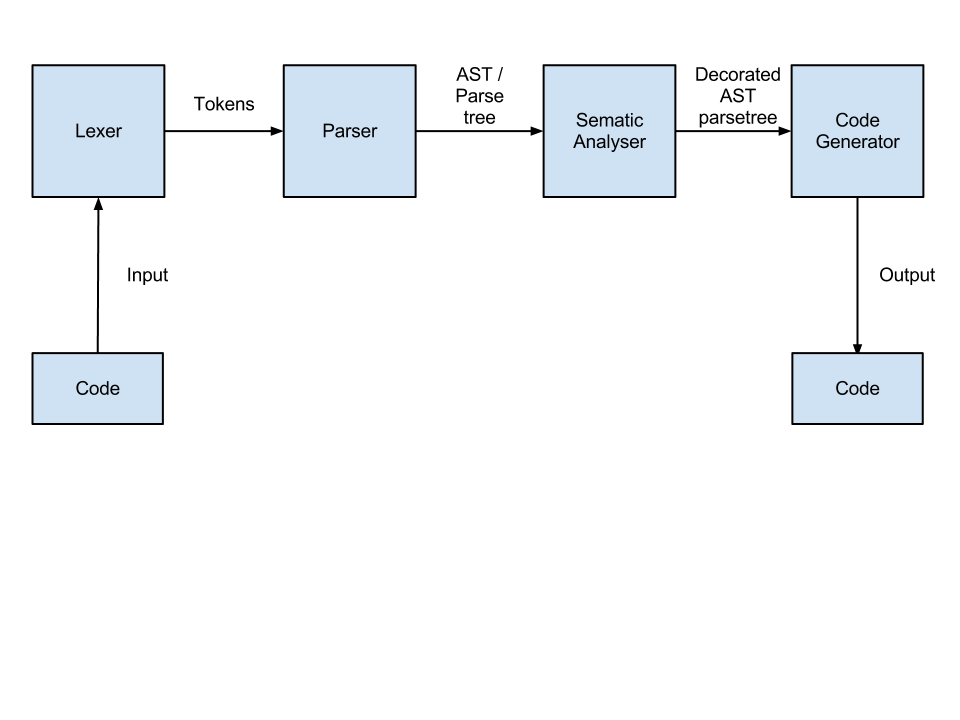
\includegraphics[width=100px]{images/Compilerconstruction.png}
		 \caption{Compiler construction}
	\label{fig:Compilerconstruction}
\end{figure}